% Options for packages loaded elsewhere
% Options for packages loaded elsewhere
\PassOptionsToPackage{unicode}{hyperref}
\PassOptionsToPackage{hyphens}{url}
%
\documentclass[
  ignorenonframetext,
  aspectratio=169,
  spanish,
]{beamer}
\newif\ifbibliography
\usepackage{pgfpages}
\setbeamertemplate{caption}[numbered]
\setbeamertemplate{caption label separator}{: }
\setbeamercolor{caption name}{fg=normal text.fg}
\beamertemplatenavigationsymbolshorizontal
% remove section numbering
\setbeamertemplate{part page}{
  \centering
  \begin{beamercolorbox}[sep=16pt,center]{part title}
    \usebeamerfont{part title}\insertpart\par
  \end{beamercolorbox}
}
\setbeamertemplate{section page}{
  \centering
  \begin{beamercolorbox}[sep=12pt,center]{section title}
    \usebeamerfont{section title}\insertsection\par
  \end{beamercolorbox}
}
\setbeamertemplate{subsection page}{
  \centering
  \begin{beamercolorbox}[sep=8pt,center]{subsection title}
    \usebeamerfont{subsection title}\insertsubsection\par
  \end{beamercolorbox}
}
% Prevent slide breaks in the middle of a paragraph
\widowpenalties 1 10000
\raggedbottom
\AtBeginPart{
  \frame{\partpage}
}
\AtBeginSection{
  \ifbibliography
  \else
    \frame{\sectionpage}
  \fi
}
\AtBeginSubsection{
  \frame{\subsectionpage}
}
\usepackage{iftex}
\ifPDFTeX
  \usepackage[T1]{fontenc}
  \usepackage[utf8]{inputenc}
  \usepackage{textcomp} % provide euro and other symbols
\else % if luatex or xetex
  \usepackage{unicode-math} % this also loads fontspec
  \defaultfontfeatures{Scale=MatchLowercase}
  \defaultfontfeatures[\rmfamily]{Ligatures=TeX,Scale=1}
\fi
\usepackage{lmodern}

\usetheme[]{default}
\usefonttheme[]{default}
\ifPDFTeX\else
  % xetex/luatex font selection
\fi
% Use upquote if available, for straight quotes in verbatim environments
\IfFileExists{upquote.sty}{\usepackage{upquote}}{}
\IfFileExists{microtype.sty}{% use microtype if available
  \usepackage[]{microtype}
  \UseMicrotypeSet[protrusion]{basicmath} % disable protrusion for tt fonts
}{}
\makeatletter
\@ifundefined{KOMAClassName}{% if non-KOMA class
  \IfFileExists{parskip.sty}{%
    \usepackage{parskip}
  }{% else
    \setlength{\parindent}{0pt}
    \setlength{\parskip}{6pt plus 2pt minus 1pt}}
}{% if KOMA class
  \KOMAoptions{parskip=half}}
\makeatother

\usepackage{color}
\usepackage{fancyvrb}
\newcommand{\VerbBar}{|}
\newcommand{\VERB}{\Verb[commandchars=\\\{\}]}
\DefineVerbatimEnvironment{Highlighting}{Verbatim}{commandchars=\\\{\}}
% Add ',fontsize=\small' for more characters per line
\usepackage{framed}
\definecolor{shadecolor}{RGB}{241,243,245}
\newenvironment{Shaded}{\begin{snugshade}}{\end{snugshade}}
\newcommand{\AlertTok}[1]{\textcolor[rgb]{0.68,0.00,0.00}{#1}}
\newcommand{\AnnotationTok}[1]{\textcolor[rgb]{0.37,0.37,0.37}{#1}}
\newcommand{\AttributeTok}[1]{\textcolor[rgb]{0.40,0.45,0.13}{#1}}
\newcommand{\BaseNTok}[1]{\textcolor[rgb]{0.68,0.00,0.00}{#1}}
\newcommand{\BuiltInTok}[1]{\textcolor[rgb]{0.00,0.23,0.31}{#1}}
\newcommand{\CharTok}[1]{\textcolor[rgb]{0.13,0.47,0.30}{#1}}
\newcommand{\CommentTok}[1]{\textcolor[rgb]{0.37,0.37,0.37}{#1}}
\newcommand{\CommentVarTok}[1]{\textcolor[rgb]{0.37,0.37,0.37}{\textit{#1}}}
\newcommand{\ConstantTok}[1]{\textcolor[rgb]{0.56,0.35,0.01}{#1}}
\newcommand{\ControlFlowTok}[1]{\textcolor[rgb]{0.00,0.23,0.31}{\textbf{#1}}}
\newcommand{\DataTypeTok}[1]{\textcolor[rgb]{0.68,0.00,0.00}{#1}}
\newcommand{\DecValTok}[1]{\textcolor[rgb]{0.68,0.00,0.00}{#1}}
\newcommand{\DocumentationTok}[1]{\textcolor[rgb]{0.37,0.37,0.37}{\textit{#1}}}
\newcommand{\ErrorTok}[1]{\textcolor[rgb]{0.68,0.00,0.00}{#1}}
\newcommand{\ExtensionTok}[1]{\textcolor[rgb]{0.00,0.23,0.31}{#1}}
\newcommand{\FloatTok}[1]{\textcolor[rgb]{0.68,0.00,0.00}{#1}}
\newcommand{\FunctionTok}[1]{\textcolor[rgb]{0.28,0.35,0.67}{#1}}
\newcommand{\ImportTok}[1]{\textcolor[rgb]{0.00,0.46,0.62}{#1}}
\newcommand{\InformationTok}[1]{\textcolor[rgb]{0.37,0.37,0.37}{#1}}
\newcommand{\KeywordTok}[1]{\textcolor[rgb]{0.00,0.23,0.31}{\textbf{#1}}}
\newcommand{\NormalTok}[1]{\textcolor[rgb]{0.00,0.23,0.31}{#1}}
\newcommand{\OperatorTok}[1]{\textcolor[rgb]{0.37,0.37,0.37}{#1}}
\newcommand{\OtherTok}[1]{\textcolor[rgb]{0.00,0.23,0.31}{#1}}
\newcommand{\PreprocessorTok}[1]{\textcolor[rgb]{0.68,0.00,0.00}{#1}}
\newcommand{\RegionMarkerTok}[1]{\textcolor[rgb]{0.00,0.23,0.31}{#1}}
\newcommand{\SpecialCharTok}[1]{\textcolor[rgb]{0.37,0.37,0.37}{#1}}
\newcommand{\SpecialStringTok}[1]{\textcolor[rgb]{0.13,0.47,0.30}{#1}}
\newcommand{\StringTok}[1]{\textcolor[rgb]{0.13,0.47,0.30}{#1}}
\newcommand{\VariableTok}[1]{\textcolor[rgb]{0.07,0.07,0.07}{#1}}
\newcommand{\VerbatimStringTok}[1]{\textcolor[rgb]{0.13,0.47,0.30}{#1}}
\newcommand{\WarningTok}[1]{\textcolor[rgb]{0.37,0.37,0.37}{\textit{#1}}}

\usepackage{longtable,booktabs,array}
\usepackage{calc} % for calculating minipage widths
\usepackage{caption}
% Make caption package work with longtable
\makeatletter
\def\fnum@table{\tablename~\thetable}
\makeatother
\usepackage{graphicx}
\makeatletter
\newsavebox\pandoc@box
\newcommand*\pandocbounded[1]{% scales image to fit in text height/width
  \sbox\pandoc@box{#1}%
  \Gscale@div\@tempa{\textheight}{\dimexpr\ht\pandoc@box+\dp\pandoc@box\relax}%
  \Gscale@div\@tempb{\linewidth}{\wd\pandoc@box}%
  \ifdim\@tempb\p@<\@tempa\p@\let\@tempa\@tempb\fi% select the smaller of both
  \ifdim\@tempa\p@<\p@\scalebox{\@tempa}{\usebox\pandoc@box}%
  \else\usebox{\pandoc@box}%
  \fi%
}
% Set default figure placement to htbp
\def\fps@figure{htbp}
\makeatother



\ifLuaTeX
\usepackage[bidi=basic]{babel}
\else
\usepackage[bidi=default]{babel}
\fi
% get rid of language-specific shorthands (see #6817):
\let\LanguageShortHands\languageshorthands
\def\languageshorthands#1{}


\setlength{\emergencystretch}{3em} % prevent overfull lines

\providecommand{\tightlist}{%
  \setlength{\itemsep}{0pt}\setlength{\parskip}{0pt}}



 


\setbeamertemplate{headline}{} % Elimina la cabecera del tema Madrid
\setbeamertemplate{section in head/foot}{} % Limpia la numeración de secciones
\renewcommand{\contentsname}{Índice}
\renewcommand{\refname}{Referencias}
\renewcommand{\figurename}{Figura}
\renewcommand{\tablename}{Tabla}
\logo{%
  \begin{tabular}{c}
    
\includegraphics[height=1.2cm]{EscudoU.png}
  \end{tabular}%
}
% --- CONFIGURACIÓN DE COLORES INSTITUCIONALES ---
\definecolor{UnicorGreen}{HTML}{024426}
\definecolor{UnicorText}{HTML}{F9F9F9}
\definecolor{UnicorWhite}{HTML}{FFFFFF}
\definecolor{UnicorGold}{HTML}{D1B061}

% Aplicación al fondo y texto general
\setbeamercolor{background canvas}{bg=UnicorGreen}
\setbeamercolor{normal text}{fg=UnicorText}

% Aplicación a títulos y cabeceras
%\setbeamercolor{title}{fg=UnicorWhite}
\setbeamercolor{frametitle}{fg=UnicorWhite}
\setbeamercolor{framesubtitle}{fg=UnicorWhite}

% Aplicación a viñetas y estructura
\setbeamercolor{structure}{fg=UnicorWhite}
\setbeamercolor{itemize item}{fg=UnicorWhite}
\setbeamercolor{itemize subitem}{fg=UnicorWhite}
\setbeamercolor{enumerate item}{fg=UnicorWhite}

% Forzar a LaTeX a repintar el texto general al iniciar el documento
\AtBeginDocument{\usebeamercolor[fg]{normal text}}

% Aplicación a hipervínculos
\hypersetup{colorlinks=true, urlcolor=UnicorGold, linkcolor=UnicorWhite}

% --- ACTIVAR ESTILO DE BLOQUES Y SOMBRAS (ESTILO MADRID) ---
\useinnertheme[shadow=true]{rounded}

% --- COLORES DEL RECUADRO DEL TÍTULO PRINCIPAL ---
% Fondo dorado con texto verde
\setbeamercolor{title}{bg=UnicorGold, fg=UnicorGreen}
\setbeamercolor{frametitle}{fg=UnicorWhite} % Mantiene el título de las diapositivas normal
\setbeamercolor{framesubtitle}{fg=UnicorWhite}

% --- COLORES PARA TEOREMAS, DEFINICIONES Y BLOQUES ---
% Título del bloque (Fondo dorado, texto verde)
\setbeamercolor{block title}{bg=UnicorGold, fg=UnicorGreen}
% Cuerpo del bloque (Fondo blanco, texto verde)
\setbeamercolor{block body}{bg=UnicorWhite, fg=UnicorGreen}

\AtBeginDocument{
  \author{%
    \begin{tabular}{c}
      Mario A. Morales Rivera \\
      \footnotesize \texttt{mamorales@correo.unicordoba.edu.co} \\
      \footnotesize Universidad de Córdoba
    \end{tabular}
  }
  \institute{}
}
% --- LIMPIAR DIAPOSITIVAS DE SECCIÓN (ELIMINAR "SECTION X") ---
\setbeamertemplate{section page}{
  \begin{center}
    \begin{beamercolorbox}[sep=12pt,center,rounded=true,shadow=true]{title}
      \usebeamerfont{title}\insertsection\par
    \end{beamercolorbox}
  \end{center}
}
\makeatletter
\@ifpackageloaded{tcolorbox}{}{\usepackage[skins,breakable]{tcolorbox}}
\@ifpackageloaded{fontawesome5}{}{\usepackage{fontawesome5}}
\definecolor{quarto-callout-color}{HTML}{909090}
\definecolor{quarto-callout-note-color}{HTML}{0758E5}
\definecolor{quarto-callout-important-color}{HTML}{CC1914}
\definecolor{quarto-callout-warning-color}{HTML}{EB9113}
\definecolor{quarto-callout-tip-color}{HTML}{00A047}
\definecolor{quarto-callout-caution-color}{HTML}{FC5300}
\definecolor{quarto-callout-color-frame}{HTML}{acacac}
\definecolor{quarto-callout-note-color-frame}{HTML}{4582ec}
\definecolor{quarto-callout-important-color-frame}{HTML}{d9534f}
\definecolor{quarto-callout-warning-color-frame}{HTML}{f0ad4e}
\definecolor{quarto-callout-tip-color-frame}{HTML}{02b875}
\definecolor{quarto-callout-caution-color-frame}{HTML}{fd7e14}
\makeatother
\makeatletter
\@ifpackageloaded{caption}{}{\usepackage{caption}}
\AtBeginDocument{%
\ifdefined\contentsname
  \renewcommand*\contentsname{Tabla de contenidos}
\else
  \newcommand\contentsname{Tabla de contenidos}
\fi
\ifdefined\listfigurename
  \renewcommand*\listfigurename{Listado de Figuras}
\else
  \newcommand\listfigurename{Listado de Figuras}
\fi
\ifdefined\listtablename
  \renewcommand*\listtablename{Listado de Tablas}
\else
  \newcommand\listtablename{Listado de Tablas}
\fi
\ifdefined\figurename
  \renewcommand*\figurename{Figura}
\else
  \newcommand\figurename{Figura}
\fi
\ifdefined\tablename
  \renewcommand*\tablename{Tabla}
\else
  \newcommand\tablename{Tabla}
\fi
}
\@ifpackageloaded{float}{}{\usepackage{float}}
\floatstyle{ruled}
\@ifundefined{c@chapter}{\newfloat{codelisting}{h}{lop}}{\newfloat{codelisting}{h}{lop}[chapter]}
\floatname{codelisting}{Listado}
\newcommand*\listoflistings{\listof{codelisting}{Listado de Listados}}
\makeatother
\makeatletter
\makeatother
\makeatletter
\@ifpackageloaded{caption}{}{\usepackage{caption}}
\@ifpackageloaded{subcaption}{}{\usepackage{subcaption}}
\makeatother

\usepackage{bookmark}
\IfFileExists{xurl.sty}{\usepackage{xurl}}{} % add URL line breaks if available
\urlstyle{same}
\hypersetup{
  pdftitle={R Como una calculadora},
  pdfauthor={Mario Morales},
  pdflang={es},
  hidelinks,
  pdfcreator={LaTeX via pandoc}}


\title{R Como una calculadora}
\subtitle{\emph{Tipos de datos }}
\author{Mario Morales}
\date{}

\begin{document}
\frame{\titlepage}

\renewcommand*\contentsname{Contenido}
\begin{frame}[allowframebreaks]
  \frametitle{Contenido}
  \setcounter{tocdepth}{3}
  \tableofcontents
\end{frame}
\setcounter{tocdepth}{3}
\tableofcontents
}

\section{Tipos de datos en R}\label{tipos-de-datos-en-r}

\begin{frame}{Tipos de datos en R}
\end{frame}

\begin{frame}[fragile]{Numéricos:}
\phantomsection\label{numuxe9ricos}
\texttt{Numeric}: Números reales, pueden tener decimales (ej: 3.14,
-2.5).

\begin{Shaded}
\begin{Highlighting}[]
\NormalTok{a}\OtherTok{=}\FloatTok{3.14} 
\FunctionTok{class}\NormalTok{(a) }
\end{Highlighting}
\end{Shaded}

\begin{verbatim}
[1] "numeric"
\end{verbatim}

\texttt{Integer}: Números enteros (ej: 5, -10).

\begin{Shaded}
\begin{Highlighting}[]
\NormalTok{b1}\OtherTok{=}\DecValTok{5}\NormalTok{L }
\FunctionTok{class}\NormalTok{(b1) }
\end{Highlighting}
\end{Shaded}

\begin{verbatim}
[1] "integer"
\end{verbatim}

\begin{Shaded}
\begin{Highlighting}[]
\NormalTok{b2}\OtherTok{=}\SpecialCharTok{{-}}\DecValTok{10}\NormalTok{L}
\FunctionTok{class}\NormalTok{(b2)}
\end{Highlighting}
\end{Shaded}

\begin{verbatim}
[1] "integer"
\end{verbatim}
\end{frame}

\begin{frame}[fragile]{}
\phantomsection\label{section}
\begin{Shaded}
\begin{Highlighting}[]
\NormalTok{b1}\OtherTok{=}\DecValTok{5} \CommentTok{\# si no se especifica como 5L lo toma como real  }
\FunctionTok{class}\NormalTok{(b1) }
\end{Highlighting}
\end{Shaded}

\begin{verbatim}
[1] "numeric"
\end{verbatim}
\end{frame}

\begin{frame}[fragile]{La diferencia está en la memoria usada}
\phantomsection\label{la-diferencia-estuxe1-en-la-memoria-usada}
\begin{Shaded}
\begin{Highlighting}[]
\CommentTok{\# Creamos un vector de 1 millón de enteros}
\NormalTok{vector\_enteros }\OtherTok{\textless{}{-}} \FunctionTok{rep}\NormalTok{(}\DecValTok{5}\NormalTok{L, }\DecValTok{1000000}\NormalTok{)}

\CommentTok{\# Creamos un vector de 1 millón de numéricos (reales)}
\NormalTok{vector\_numericos }\OtherTok{\textless{}{-}} \FunctionTok{rep}\NormalTok{(}\DecValTok{5}\NormalTok{, }\DecValTok{1000000}\NormalTok{)}

\FunctionTok{c}\NormalTok{(}\StringTok{"Entero"}\OtherTok{=}\FunctionTok{object.size}\NormalTok{(vector\_enteros),}\StringTok{"Real"}\OtherTok{=}\FunctionTok{object.size}\NormalTok{(vector\_numericos) ) }
\end{Highlighting}
\end{Shaded}

\begin{verbatim}
 Entero    Real 
4000048 8000048 
\end{verbatim}
\end{frame}

\begin{frame}[fragile]{}
\phantomsection\label{section-1}
\texttt{Complex}: Números complejos (ej: 3+2i).

\begin{Shaded}
\begin{Highlighting}[]
\NormalTok{c1}\OtherTok{=} \DecValTok{3}\SpecialCharTok{+}\DecValTok{2}\NormalTok{i}
\FunctionTok{class}\NormalTok{(c1) }
\end{Highlighting}
\end{Shaded}

\begin{verbatim}
[1] "complex"
\end{verbatim}
\end{frame}

\begin{frame}[fragile]{Caracteres:}
\phantomsection\label{caracteres}
\texttt{Character}: Texto, siempre encerrado entre comillas (ej: ``Trat
1'', ``Análisis de datos'').

\begin{Shaded}
\begin{Highlighting}[]
\NormalTok{ch}\OtherTok{=}\StringTok{"Trat 1"}  
\FunctionTok{class}\NormalTok{(ch) }
\end{Highlighting}
\end{Shaded}

\begin{verbatim}
[1] "character"
\end{verbatim}
\end{frame}

\begin{frame}[fragile]{Lógicos:}
\phantomsection\label{luxf3gicos}
\texttt{Logical}: Valores booleanos, \texttt{TRUE} o \texttt{FALSE}.

\begin{Shaded}
\begin{Highlighting}[]
\NormalTok{l}\OtherTok{=}\ConstantTok{TRUE}  
\FunctionTok{class}\NormalTok{(l)  }
\end{Highlighting}
\end{Shaded}

\begin{verbatim}
[1] "logical"
\end{verbatim}
\end{frame}

\begin{frame}[fragile]{Funciones \texttt{is.}}
\phantomsection\label{funciones-is.}
Se usan para indagar el tipo de dato que es un objeto

\begin{Shaded}
\begin{Highlighting}[]
\FunctionTok{is.numeric}\NormalTok{(b2)}
\end{Highlighting}
\end{Shaded}

\begin{verbatim}
[1] TRUE
\end{verbatim}

\begin{Shaded}
\begin{Highlighting}[]
\FunctionTok{is.logical}\NormalTok{(ch)}
\end{Highlighting}
\end{Shaded}

\begin{verbatim}
[1] FALSE
\end{verbatim}

\begin{tcolorbox}[enhanced jigsaw, leftrule=.75mm, toptitle=1mm, breakable, title=\textcolor{quarto-callout-important-color}{\faExclamation}\hspace{0.5em}{Importante}, colback=white, toprule=.15mm, opacityback=0, arc=.35mm, colframe=quarto-callout-important-color-frame, colbacktitle=quarto-callout-important-color!10!white, bottomtitle=1mm, left=2mm, rightrule=.15mm, opacitybacktitle=0.6, coltitle=black, bottomrule=.15mm, titlerule=0mm]

Observe que estas funciones regresan un valor lógico (\texttt{logical})

\end{tcolorbox}
\end{frame}

\begin{frame}{Tipos de datos básicos en R II}
\phantomsection\label{tipos-de-datos-buxe1sicos-en-r-ii}
\begin{block}{Factores:}
\phantomsection\label{factores}
Factor: Categorías o niveles de una variable, utilizados para variables
cualitativas (ej: ``Hombre'', ``Mujer'').
\end{block}
\end{frame}

\begin{frame}{Estructuras de Datos}
\phantomsection\label{estructuras-de-datos}
\begin{block}{Vectores:}
\phantomsection\label{vectores}
Secuencia de elementos del \textbf{mismo tipo} (numéricos, caracteres,
lógicos).
\end{block}

\begin{block}{Matrices:}
\phantomsection\label{matrices}
Arreglos bidimensionales de \emph{elementos} del mismo tipo.
\end{block}

\begin{block}{Data frames:}
\phantomsection\label{data-frames}
Estructura de datos similar a una hoja de cálculo, con columnas de
(posiblemete) diferentes tipos.
\end{block}
\end{frame}

\begin{frame}{Estructuras de Datos (II)}
\phantomsection\label{estructuras-de-datos-ii}
\begin{block}{Listas:}
\phantomsection\label{listas}
Objetos que pueden contener diferentes tipos de elementos, incluyendo
otros objetos.
\end{block}
\end{frame}

\begin{frame}[fragile]{Conocer el tipo de dato}
\phantomsection\label{conocer-el-tipo-de-dato}
\begin{Shaded}
\begin{Highlighting}[numbers=left,,]
\FunctionTok{class}\NormalTok{(}\FloatTok{3.5}\NormalTok{)}
\FunctionTok{class}\NormalTok{(}\DecValTok{3}\NormalTok{)}
\FunctionTok{class}\NormalTok{(}\DecValTok{1}\SpecialCharTok{:}\DecValTok{3}\NormalTok{)}
\FunctionTok{class}\NormalTok{(}\DecValTok{2}\NormalTok{L)}
\end{Highlighting}
\end{Shaded}

\begin{Shaded}
\begin{Highlighting}[numbers=left,,]
\FunctionTok{class}\NormalTok{(}\DecValTok{3}\SpecialCharTok{+}\DecValTok{2}\NormalTok{i)}
\FunctionTok{class}\NormalTok{(}\StringTok{\textquotesingle{}Hola mundo\textquotesingle{}}\NormalTok{)}
\FunctionTok{class}\NormalTok{(}\StringTok{"Hola mundo"}\NormalTok{)}
\FunctionTok{class}\NormalTok{(}\ConstantTok{TRUE}\NormalTok{)}
\FunctionTok{class}\NormalTok{(}\ConstantTok{FALSE}\NormalTok{) }
\FunctionTok{class}\NormalTok{(}\ConstantTok{NA}\NormalTok{)  }
\end{Highlighting}
\end{Shaded}
\end{frame}

\begin{frame}[fragile]{Funciones \texttt{is}}
\phantomsection\label{funciones-is}
Estas funciones regresan \texttt{TRUE} si el objeto es del tipo indicado
después del punto y \texttt{FALSE} en otro caso.

\begin{Shaded}
\begin{Highlighting}[]
\FunctionTok{is.numeric}\NormalTok{(}\DecValTok{3}\NormalTok{)}
\FunctionTok{is.integer}\NormalTok{(}\DecValTok{3}\NormalTok{) }
\FunctionTok{is.integer}\NormalTok{(}\DecValTok{3}\NormalTok{L)}
\FunctionTok{is.numeric}\NormalTok{(}\StringTok{"M"}\NormalTok{)}
\FunctionTok{is.character}\NormalTok{(}\StringTok{"M"}\NormalTok{)}
\FunctionTok{is.logical}\NormalTok{(}\ConstantTok{TRUE}\NormalTok{)}
\FunctionTok{is.logical}\NormalTok{(}\ConstantTok{NA}\NormalTok{)}
\FunctionTok{is.logical}\NormalTok{(}\StringTok{"M"}\NormalTok{)}
\end{Highlighting}
\end{Shaded}
\end{frame}

\begin{frame}[fragile]{Aplicación}
\phantomsection\label{aplicaciuxf3n}
Código que toma un objeto \texttt{x}, si es numérico eleva al cuadrado,
en caso contrario manda un mensaje de error.

\begin{Shaded}
\begin{Highlighting}[numbers=left,,]
\NormalTok{x}\OtherTok{=}\StringTok{"M"}
\CommentTok{\#x=4}
\ControlFlowTok{if}\NormalTok{(}\FunctionTok{is.numeric}\NormalTok{(x))\{}
\NormalTok{x}\SpecialCharTok{\^{}}\DecValTok{2}  
\NormalTok{\}}\ControlFlowTok{else}\NormalTok{\{ }\FunctionTok{cat}\NormalTok{(}\StringTok{"Se necesita un numérico"}\NormalTok{)}
\NormalTok{\}}
\end{Highlighting}
\end{Shaded}

\begin{verbatim}
Se necesita un numérico
\end{verbatim}
\end{frame}

\section{Usando R como una
calculadora}\label{usando-r-como-una-calculadora}

\begin{frame}{R como una calculadora}
\phantomsection\label{r-como-una-calculadora}
\begin{block}{Qué aprenderemos:}
\phantomsection\label{quuxe9-aprenderemos}
\begin{itemize}
\tightlist
\item
  Poder usar R como calculadora científica
\item
  Poder asignar una variable y ver su valor
\end{itemize}
\end{block}
\end{frame}

\begin{frame}[fragile]{Operaciones}
\phantomsection\label{operaciones}
\begin{Shaded}
\begin{Highlighting}[]
\DecValTok{2}\SpecialCharTok{+}\DecValTok{2} \CommentTok{\# suma}
\end{Highlighting}
\end{Shaded}

\begin{verbatim}
[1] 4
\end{verbatim}

\begin{Shaded}
\begin{Highlighting}[]
\DecValTok{5{-}3} \CommentTok{\# resta }
\end{Highlighting}
\end{Shaded}

\begin{verbatim}
[1] 2
\end{verbatim}

\begin{Shaded}
\begin{Highlighting}[]
\DecValTok{3}\SpecialCharTok{*}\DecValTok{5} \CommentTok{\# producto}
\end{Highlighting}
\end{Shaded}

\begin{verbatim}
[1] 15
\end{verbatim}
\end{frame}

\begin{frame}[fragile]{Potencia}
\phantomsection\label{potencia}
\begin{Shaded}
\begin{Highlighting}[]
\DecValTok{2}\SpecialCharTok{\^{}}\DecValTok{2} \CommentTok{\# potencia  }
\end{Highlighting}
\end{Shaded}

\begin{verbatim}
[1] 4
\end{verbatim}

\begin{Shaded}
\begin{Highlighting}[]
\DecValTok{9}\SpecialCharTok{\^{}}\NormalTok{(}\DecValTok{1}\SpecialCharTok{/}\DecValTok{2}\NormalTok{) }
\end{Highlighting}
\end{Shaded}

\begin{verbatim}
[1] 3
\end{verbatim}

\begin{Shaded}
\begin{Highlighting}[]
\DocumentationTok{\#\#\# también se puede usar **}
\DecValTok{2}\SpecialCharTok{**}\DecValTok{2}
\end{Highlighting}
\end{Shaded}

\begin{verbatim}
[1] 4
\end{verbatim}

\begin{Shaded}
\begin{Highlighting}[]
\DecValTok{9}\SpecialCharTok{**}\NormalTok{(}\DecValTok{1}\SpecialCharTok{/}\DecValTok{2}\NormalTok{)}
\end{Highlighting}
\end{Shaded}

\begin{verbatim}
[1] 3
\end{verbatim}
\end{frame}

\begin{frame}[fragile]{Cociente}
\phantomsection\label{cociente}
\begin{Shaded}
\begin{Highlighting}[]
\DecValTok{6}\SpecialCharTok{/}\DecValTok{3}
\end{Highlighting}
\end{Shaded}

\begin{verbatim}
[1] 2
\end{verbatim}
\end{frame}

\begin{frame}[fragile]{Residuo de la división}
\phantomsection\label{residuo-de-la-divisiuxf3n}
\begin{Shaded}
\begin{Highlighting}[]
\DecValTok{6}\SpecialCharTok{\%\%}\DecValTok{2}
\end{Highlighting}
\end{Shaded}

\begin{verbatim}
[1] 0
\end{verbatim}

\begin{Shaded}
\begin{Highlighting}[]
\DecValTok{10}\SpecialCharTok{\%\%}\DecValTok{4}
\end{Highlighting}
\end{Shaded}

\begin{verbatim}
[1] 2
\end{verbatim}
\end{frame}

\begin{frame}[fragile]{parte entera de la división}
\phantomsection\label{parte-entera-de-la-divisiuxf3n}
\begin{Shaded}
\begin{Highlighting}[]
\DecValTok{6}\SpecialCharTok{\%/\%}\DecValTok{4}
\end{Highlighting}
\end{Shaded}

\begin{verbatim}
[1] 1
\end{verbatim}
\end{frame}

\begin{frame}[fragile]{Ejemplo de aplicación}
\phantomsection\label{ejemplo-de-aplicaciuxf3n}
El siguiente código genera un vector \texttt{x} numérico de longitud
\(n\), escribir el código \texttt{R} que indique si el número \(n\) es
par o es impar.

Ayuda: La longitud de un vector \texttt{x} se obtiene con
\texttt{length(x)}

\begin{Shaded}
\begin{Highlighting}[]
\NormalTok{x}\OtherTok{=}\FunctionTok{round}\NormalTok{(}\FunctionTok{rnorm}\NormalTok{(}\FunctionTok{sample}\NormalTok{(}\DecValTok{10}\SpecialCharTok{:}\DecValTok{50}\NormalTok{,}\DecValTok{1}\NormalTok{)))}
\end{Highlighting}
\end{Shaded}

La longitud de \texttt{x} es: 35

\begin{Shaded}
\begin{Highlighting}[]
\NormalTok{n}\OtherTok{=}\FunctionTok{length}\NormalTok{(x)}
\ControlFlowTok{if}\NormalTok{(n}\SpecialCharTok{\%\%}\DecValTok{2}\SpecialCharTok{==}\DecValTok{0}\NormalTok{)\{}\FunctionTok{cat}\NormalTok{(}\StringTok{"n es par"}\NormalTok{)}
\NormalTok{  \}}\ControlFlowTok{else}\NormalTok{\{}\FunctionTok{cat}\NormalTok{(}\StringTok{"n es impar"}\NormalTok{)\}}
\end{Highlighting}
\end{Shaded}

\begin{verbatim}
n es impar
\end{verbatim}
\end{frame}

\begin{frame}[fragile]{Varias operaciones juntas}
\phantomsection\label{varias-operaciones-juntas}
\begin{Shaded}
\begin{Highlighting}[]
\DecValTok{4{-}2}\SpecialCharTok{*}\DecValTok{3}\SpecialCharTok{\^{}}\DecValTok{2} 
\end{Highlighting}
\end{Shaded}

\begin{verbatim}
[1] -14
\end{verbatim}
\end{frame}

\begin{frame}[fragile]{Orden de las operaciones}
\phantomsection\label{orden-de-las-operaciones}
\begin{Shaded}
\begin{Highlighting}[]
\CommentTok{\# el orden de las operaciones se altera con parentices  }
\NormalTok{(}\DecValTok{4{-}2}\NormalTok{)}\SpecialCharTok{*}\DecValTok{3}\SpecialCharTok{\^{}}\DecValTok{2}
\end{Highlighting}
\end{Shaded}

\begin{verbatim}
[1] 18
\end{verbatim}
\end{frame}

\begin{frame}[fragile]{Tres formas de asignar valores a un objeto}
\phantomsection\label{tres-formas-de-asignar-valores-a-un-objeto}
\begin{itemize}
\tightlist
\item
  La primera forma es usando \texttt{\textless{}-}
\end{itemize}

\begin{Shaded}
\begin{Highlighting}[]
\NormalTok{x}\OtherTok{\textless{}{-}}\DecValTok{10}
\NormalTok{x}
\end{Highlighting}
\end{Shaded}

\begin{verbatim}
[1] 10
\end{verbatim}

\begin{itemize}
\tightlist
\item
  La segunda forma es usando \texttt{=}
\end{itemize}

\begin{Shaded}
\begin{Highlighting}[]
\NormalTok{y}\OtherTok{=}\DecValTok{2}
\NormalTok{y}
\end{Highlighting}
\end{Shaded}

\begin{verbatim}
[1] 2
\end{verbatim}

\begin{itemize}
\tightlist
\item
  La tercera forma es usando \texttt{-\textgreater{}}
\end{itemize}

\begin{Shaded}
\begin{Highlighting}[]
\DecValTok{10}\OtherTok{{-}\textgreater{}}\NormalTok{x}
\end{Highlighting}
\end{Shaded}
\end{frame}

\begin{frame}[fragile]{Ejemplo: Valor presente}
\phantomsection\label{ejemplo-valor-presente}
Suponga que queremos hacer un programa para estimar el valor presente de
\(\$ 100\) recibidos en dos años con una tasa de descuento anual del
\(8\%\). La fórmula relacionada se muestra a continuación
\[Pv=\frac{Fv}{(1+R)^n}\]

\begin{Shaded}
\begin{Highlighting}[]
\NormalTok{Fv}\OtherTok{=}\DecValTok{100}
\NormalTok{R}\OtherTok{=}\FloatTok{0.08}
\NormalTok{n}\OtherTok{=}\DecValTok{2}
\end{Highlighting}
\end{Shaded}
\end{frame}

\begin{frame}[fragile]{Ejemplo: Valor presente (cont)}
\phantomsection\label{ejemplo-valor-presente-cont}
\begin{Shaded}
\begin{Highlighting}[]
\NormalTok{Fv}\SpecialCharTok{/}\NormalTok{(}\DecValTok{1}\SpecialCharTok{+}\NormalTok{R)}\SpecialCharTok{\^{}}\DecValTok{2}
\end{Highlighting}
\end{Shaded}

\begin{verbatim}
[1] 85.73388
\end{verbatim}

\begin{Shaded}
\begin{Highlighting}[]
\NormalTok{Fv}\SpecialCharTok{/}\NormalTok{(}\DecValTok{1}\SpecialCharTok{+}\NormalTok{R)}\SpecialCharTok{\^{}}\DecValTok{2}\OtherTok{{-}\textgreater{}}\NormalTok{Pv}
\NormalTok{Pv}
\end{Highlighting}
\end{Shaded}

\begin{verbatim}
[1] 85.73388
\end{verbatim}
\end{frame}

\begin{frame}[fragile]{Vectores}
\phantomsection\label{vectores-1}
Para asignar un conjunto de valores a un vector, usamos
\texttt{c(n1,n2,...,nk)}, \texttt{c} es una abreviatura de concatenar
\texttt{concatenate}.

\begin{Shaded}
\begin{Highlighting}[]
\NormalTok{x}\OtherTok{\textless{}{-}}\FunctionTok{c}\NormalTok{(}\DecValTok{1}\NormalTok{,}\FloatTok{2.6}\NormalTok{,}\FloatTok{4.3}\NormalTok{,}\FloatTok{5.25}\NormalTok{)}
\end{Highlighting}
\end{Shaded}

Para asignar un conjunto de enteros consecutivos
\texttt{secuencia\ regular}, podríamos usar \texttt{n1:n2}, como
\texttt{1:10}

\begin{Shaded}
\begin{Highlighting}[]
\NormalTok{y}\OtherTok{\textless{}{-}}\DecValTok{1}\SpecialCharTok{:}\DecValTok{50}
\NormalTok{y}
\end{Highlighting}
\end{Shaded}

\begin{verbatim}
 [1]  1  2  3  4  5  6  7  8  9 10 11 12 13 14 15 16 17 18 19 20 21 22 23 24 25
[26] 26 27 28 29 30 31 32 33 34 35 36 37 38 39 40 41 42 43 44 45 46 47 48 49 50
\end{verbatim}
\end{frame}

\begin{frame}[fragile]{Vectores (cont.)}
\phantomsection\label{vectores-cont.}
\begin{Shaded}
\begin{Highlighting}[]
\DocumentationTok{\#\# desde 5 hasta 1 disminuyendo de 1 en 1 }
\NormalTok{x}\OtherTok{\textless{}{-}}\DecValTok{5}\SpecialCharTok{:}\DecValTok{1} 
\NormalTok{x}\OtherTok{\textless{}{-}}\FunctionTok{rev}\NormalTok{(}\DecValTok{1}\SpecialCharTok{:}\DecValTok{5}\NormalTok{)  }
\end{Highlighting}
\end{Shaded}

R distingue entre mayúsculas y minúsculas, lo que significa que la
\texttt{X} mayúscula y la \texttt{x} minúscula son variables diferentes.

\begin{Shaded}
\begin{Highlighting}[]
\NormalTok{x}\OtherTok{=}\DecValTok{10}
\NormalTok{X}
\end{Highlighting}
\end{Shaded}
\end{frame}

\begin{frame}[fragile]{Funciones \texttt{ls()} and \texttt{rm()}}
\phantomsection\label{funciones-ls-and-rm}
A veces necesitamos verificar todas las variables existentes (objetos)
en la memoria. para eso usamos la función \texttt{ls()}.

\begin{Shaded}
\begin{Highlighting}[]
\FunctionTok{ls}\NormalTok{()}
\end{Highlighting}
\end{Shaded}

\begin{verbatim}
 [1] "a"  "b1" "b2" "c1" "ch" "Fv" "l"  "n"  "Pv" "R"  "x"  "y" 
\end{verbatim}

Cuando ya no se necesita una variable, podemos eliminarla de la memoria
con la función \texttt{rm()}

\begin{Shaded}
\begin{Highlighting}[]
\FunctionTok{rm}\NormalTok{(z)}
\FunctionTok{ls}\NormalTok{()}
\end{Highlighting}
\end{Shaded}

\begin{verbatim}
 [1] "a"  "b1" "b2" "c1" "ch" "Fv" "l"  "n"  "Pv" "R"  "x"  "y" 
\end{verbatim}
\end{frame}

\begin{frame}[fragile]{Borrar más de una}
\phantomsection\label{borrar-muxe1s-de-una}
\begin{Shaded}
\begin{Highlighting}[]
\CommentTok{\# borrar mas de una }
\CommentTok{\#rm(y,y\_g,ycs,yg)}
\FunctionTok{ls}\NormalTok{()}
\end{Highlighting}
\end{Shaded}

\begin{verbatim}
 [1] "a"  "b1" "b2" "c1" "ch" "Fv" "l"  "n"  "Pv" "R"  "x"  "y" 
\end{verbatim}

Para eliminar todas las variables (objetos), tenemos el siguiente código

\begin{Shaded}
\begin{Highlighting}[]
\FunctionTok{rm}\NormalTok{(}\AttributeTok{list=}\FunctionTok{ls}\NormalTok{())}
\FunctionTok{ls}\NormalTok{()}
\end{Highlighting}
\end{Shaded}

\begin{verbatim}
character(0)
\end{verbatim}
\end{frame}

\begin{frame}[fragile]{Imprimir el contenido de un objeto.}
\phantomsection\label{imprimir-el-contenido-de-un-objeto.}
Para imprimir una variable de carácter (es decir, una cadena) en la
pantalla, podríamos usar las funciones \texttt{cat()} o
\texttt{print()}. Recuerde encerrar las cadenas entre comillas simples o
dobles.

\begin{Shaded}
\begin{Highlighting}[]
\FunctionTok{cat}\NormalTok{(}\StringTok{\textquotesingle{}Hola R!!!!\textquotesingle{}}\NormalTok{)}
\end{Highlighting}
\end{Shaded}

\begin{verbatim}
Hola R!!!!
\end{verbatim}

\begin{Shaded}
\begin{Highlighting}[]
\FunctionTok{print}\NormalTok{(}\StringTok{\textquotesingle{}Hola R!!!!\textquotesingle{}}\NormalTok{)}
\end{Highlighting}
\end{Shaded}

\begin{verbatim}
[1] "Hola R!!!!"
\end{verbatim}
\end{frame}

\begin{frame}[fragile]{Imprimir el contenido de un objeto.}
\phantomsection\label{imprimir-el-contenido-de-un-objeto.-1}
\begin{Shaded}
\begin{Highlighting}[]
\FunctionTok{cat}\NormalTok{(}\StringTok{\textquotesingle{}Hola R!!!! }\SpecialCharTok{\textbackslash{}n}\StringTok{ }\SpecialCharTok{\textbackslash{}n}\StringTok{ }\SpecialCharTok{\textbackslash{}n}\StringTok{\textquotesingle{}}\NormalTok{) }\CommentTok{\# \textbackslash{}n es para nueva linea}
\end{Highlighting}
\end{Shaded}

\begin{verbatim}
Hola R!!!! 
 
 
\end{verbatim}

\begin{Shaded}
\begin{Highlighting}[]
\FunctionTok{print}\NormalTok{(}\StringTok{\textquotesingle{}Hola R!!!!\textquotesingle{}}\NormalTok{)}
\end{Highlighting}
\end{Shaded}

\begin{verbatim}
[1] "Hola R!!!!"
\end{verbatim}

\begin{Shaded}
\begin{Highlighting}[]
\FunctionTok{print}\NormalTok{(}\StringTok{\textquotesingle{}Hola R!!!!  }\SpecialCharTok{\textbackslash{}n}\StringTok{ }\SpecialCharTok{\textbackslash{}n}\StringTok{ }\SpecialCharTok{\textbackslash{}n}\StringTok{ \textquotesingle{}}\NormalTok{)}
\end{Highlighting}
\end{Shaded}

\begin{verbatim}
[1] "Hola R!!!!  \n \n \n "
\end{verbatim}

\begin{Shaded}
\begin{Highlighting}[]
\FunctionTok{print}\NormalTok{(}\StringTok{\textquotesingle{}Hola R!!!!\textquotesingle{}}\NormalTok{) }\CommentTok{\# \textbackslash{}n es para nueva linea}
\end{Highlighting}
\end{Shaded}

\begin{verbatim}
[1] "Hola R!!!!"
\end{verbatim}
\end{frame}

\section{Secuencias}\label{secuencias}

\begin{frame}[fragile]{La función \texttt{seq()}}
\phantomsection\label{la-funciuxf3n-seq}
La función \texttt{seq()} se utiliza para generar un conjunto de valores
con cierto patrón.

\begin{Shaded}
\begin{Highlighting}[]
\FunctionTok{seq}\NormalTok{(}\DecValTok{1}\NormalTok{,}\DecValTok{19}\NormalTok{,}\AttributeTok{by=}\DecValTok{2}\NormalTok{)}
\end{Highlighting}
\end{Shaded}

\begin{verbatim}
 [1]  1  3  5  7  9 11 13 15 17 19
\end{verbatim}

\begin{Shaded}
\begin{Highlighting}[]
\NormalTok{x}\OtherTok{\textless{}{-}}\FunctionTok{seq}\NormalTok{(}\DecValTok{1}\NormalTok{, }\DecValTok{11}\NormalTok{, }\AttributeTok{by =}\NormalTok{ pi) }
\NormalTok{x}
\end{Highlighting}
\end{Shaded}

\begin{verbatim}
[1]  1.000000  4.141593  7.283185 10.424778
\end{verbatim}

El comando completo tiene el siguiente formato.

\begin{Shaded}
\begin{Highlighting}[]
\FunctionTok{seq}\NormalTok{(}\AttributeTok{from=}\DecValTok{1}\NormalTok{,}\AttributeTok{to=}\DecValTok{3}\NormalTok{, }\AttributeTok{by=}\FloatTok{0.5}\NormalTok{)}
\end{Highlighting}
\end{Shaded}

\begin{verbatim}
[1] 1.0 1.5 2.0 2.5 3.0
\end{verbatim}
\end{frame}

\begin{frame}[fragile]{La función rep()}
\phantomsection\label{la-funciuxf3n-rep}
La función rep() se usa para repetir el mismo valor \(n\) veces, como se
muestra a continuación.

\begin{Shaded}
\begin{Highlighting}[]
\FunctionTok{rep}\NormalTok{(}\DecValTok{5}\NormalTok{,}\DecValTok{10}\NormalTok{)}
\end{Highlighting}
\end{Shaded}

\begin{verbatim}
 [1] 5 5 5 5 5 5 5 5 5 5
\end{verbatim}

\begin{Shaded}
\begin{Highlighting}[]
\FunctionTok{rep}\NormalTok{(}\FunctionTok{c}\NormalTok{(}\DecValTok{1}\NormalTok{,}\DecValTok{2}\NormalTok{,}\DecValTok{3}\NormalTok{),}\DecValTok{5}\NormalTok{)}
\end{Highlighting}
\end{Shaded}

\begin{verbatim}
 [1] 1 2 3 1 2 3 1 2 3 1 2 3 1 2 3
\end{verbatim}

\begin{Shaded}
\begin{Highlighting}[]
\FunctionTok{rep}\NormalTok{(}\FunctionTok{c}\NormalTok{(}\DecValTok{1}\NormalTok{,}\DecValTok{2}\NormalTok{,}\DecValTok{3}\NormalTok{),}\AttributeTok{each=}\DecValTok{5}\NormalTok{) }
\end{Highlighting}
\end{Shaded}

\begin{verbatim}
 [1] 1 1 1 1 1 2 2 2 2 2 3 3 3 3 3
\end{verbatim}
\end{frame}

\begin{frame}[fragile]{La función length()}
\phantomsection\label{la-funciuxf3n-length}
Para encontrar el número de valores (observaciones) que tiene un vector,
aplicamos la función \texttt{length()}, como se muestra a continuación.

\begin{Shaded}
\begin{Highlighting}[]
\FunctionTok{length}\NormalTok{(x)}
\end{Highlighting}
\end{Shaded}

\begin{verbatim}
[1] 4
\end{verbatim}

\begin{Shaded}
\begin{Highlighting}[]
\FunctionTok{length}\NormalTok{(}\FunctionTok{rep}\NormalTok{(}\DecValTok{5}\NormalTok{,}\DecValTok{7}\NormalTok{))}
\end{Highlighting}
\end{Shaded}

\begin{verbatim}
[1] 7
\end{verbatim}
\end{frame}

\begin{frame}[fragile]{Enfoque de posición}
\phantomsection\label{enfoque-de-posiciuxf3n}
Hay dos formas de entregar datos a una función: por \textbf{posición} y
por \textbf{palabra clave}. Para la función \texttt{seq()}, su formato
es \texttt{seq(from,to,by)}. En el siguiente código de una línea, usamos
la forma de posición. En otras palabras, el valor del argumento de
entrada depende de su posición en el conjunto de valores de entrada
entregados.

\begin{Shaded}
\begin{Highlighting}[]
\NormalTok{x}\OtherTok{\textless{}{-}}\FunctionTok{seq}\NormalTok{(}\DecValTok{1}\NormalTok{,}\DecValTok{3}\NormalTok{,}\FloatTok{0.5}\NormalTok{)}
\end{Highlighting}
\end{Shaded}
\end{frame}

\begin{frame}[fragile]{Enfoque de palabra clave}
\phantomsection\label{enfoque-de-palabra-clave}
Para el enfoque de \textbf{palabra clave}, agregamos una palabra clave
delante de cada valor de entrada, como \texttt{from=1}. Una ventaja del
enfoque de palabra clave es que el orden de los valores de entrada no
influye; Por lo tanto, las siguientes tres lineas son equivalentes.

\begin{Shaded}
\begin{Highlighting}[]
\FunctionTok{seq}\NormalTok{(}\AttributeTok{from=}\DecValTok{1}\NormalTok{,}\AttributeTok{to=}\DecValTok{3}\NormalTok{,}\AttributeTok{by=}\FloatTok{0.5}\NormalTok{) }\CommentTok{\# son equivalentes }
\end{Highlighting}
\end{Shaded}

\begin{verbatim}
[1] 1.0 1.5 2.0 2.5 3.0
\end{verbatim}

\begin{Shaded}
\begin{Highlighting}[]
\FunctionTok{seq}\NormalTok{(}\AttributeTok{to=}\DecValTok{3}\NormalTok{,}\AttributeTok{from=}\DecValTok{1}\NormalTok{,}\AttributeTok{by=}\FloatTok{0.5}\NormalTok{)}
\end{Highlighting}
\end{Shaded}

\begin{verbatim}
[1] 1.0 1.5 2.0 2.5 3.0
\end{verbatim}

\begin{Shaded}
\begin{Highlighting}[]
\FunctionTok{seq}\NormalTok{(}\AttributeTok{by=}\FloatTok{0.5}\NormalTok{,}\AttributeTok{to=}\DecValTok{3}\NormalTok{,}\AttributeTok{from=}\DecValTok{1}\NormalTok{)}
\end{Highlighting}
\end{Shaded}

\begin{verbatim}
[1] 1.0 1.5 2.0 2.5 3.0
\end{verbatim}

\begin{block}{Entrada de datos con \texttt{scan}}
\phantomsection\label{entrada-de-datos-con-scan}
Otra manera fácil de ingresar datos desde el teclado es usar la funcion
\texttt{escan()}

\begin{Shaded}
\begin{Highlighting}[]
\CommentTok{\# en los notebooks no trabaja }
\NormalTok{x}\OtherTok{\textless{}{-}}\FunctionTok{scan}\NormalTok{()}
\DecValTok{1}
\end{Highlighting}
\end{Shaded}

\begin{verbatim}
[1] 1
\end{verbatim}

\begin{Shaded}
\begin{Highlighting}[]
\DecValTok{4}
\end{Highlighting}
\end{Shaded}

\begin{verbatim}
[1] 4
\end{verbatim}

\begin{Shaded}
\begin{Highlighting}[]
\DecValTok{5}
\end{Highlighting}
\end{Shaded}

\begin{verbatim}
[1] 5
\end{verbatim}

\begin{Shaded}
\begin{Highlighting}[]
\DecValTok{1}
\end{Highlighting}
\end{Shaded}

\begin{verbatim}
[1] 1
\end{verbatim}

\begin{Shaded}
\begin{Highlighting}[]
\DecValTok{3}
\end{Highlighting}
\end{Shaded}

\begin{verbatim}
[1] 3
\end{verbatim}

\begin{Shaded}
\begin{Highlighting}[]
\CommentTok{\#x=scan()}
\CommentTok{\#1 4 }
\CommentTok{\#2 5 }
\CommentTok{\#4 1 }
\CommentTok{\#5 7 }
\CommentTok{\#8 9 }
\CommentTok{\#1 2 }
\CommentTok{\#matrix(x,nrow=6,byrow = TRUE)}
\end{Highlighting}
\end{Shaded}

\begin{Shaded}
\begin{Highlighting}[]
\FunctionTok{print}\NormalTok{(x)}
\end{Highlighting}
\end{Shaded}

\begin{verbatim}
numeric(0)
\end{verbatim}
\end{block}
\end{frame}

\begin{frame}[fragile]{Residuo de la división}
\phantomsection\label{residuo-de-la-divisiuxf3n-1}
El operador \texttt{\%\%} regresa el residuo de la división

\begin{Shaded}
\begin{Highlighting}[]
\CommentTok{\# residuo de la división }
\DecValTok{7}\SpecialCharTok{\%\%}\DecValTok{2}
\end{Highlighting}
\end{Shaded}

\begin{verbatim}
[1] 1
\end{verbatim}

\begin{Shaded}
\begin{Highlighting}[]
\CommentTok{\# ¿qué valor regresa la operación?  }
\DecValTok{9}\SpecialCharTok{\%\%}\DecValTok{3} 
\end{Highlighting}
\end{Shaded}

\begin{verbatim}
[1] 0
\end{verbatim}
\end{frame}

\begin{frame}[fragile]{Parte entera de la división}
\phantomsection\label{parte-entera-de-la-divisiuxf3n-1}
El operador \texttt{\%/\%} regresa la parte entera de la división

\begin{Shaded}
\begin{Highlighting}[]
\DecValTok{7}\SpecialCharTok{\%/\%}\DecValTok{2}
\end{Highlighting}
\end{Shaded}

\begin{verbatim}
[1] 3
\end{verbatim}
\end{frame}

\section{Funciones}\label{funciones}

\begin{frame}[fragile]{Raíz cuadrada}
\phantomsection\label{rauxedz-cuadrada}
Calcular la raíz cuadrada de 5, es decir, \(\sqrt{5}\)

\begin{Shaded}
\begin{Highlighting}[]
\FunctionTok{sqrt}\NormalTok{(}\DecValTok{5}\NormalTok{)}
\end{Highlighting}
\end{Shaded}

\begin{verbatim}
[1] 2.236068
\end{verbatim}

\begin{Shaded}
\begin{Highlighting}[]
\FunctionTok{sqrt}\NormalTok{(}\DecValTok{9}\NormalTok{)}
\end{Highlighting}
\end{Shaded}

\begin{verbatim}
[1] 3
\end{verbatim}

\begin{Shaded}
\begin{Highlighting}[]
\FunctionTok{sqrt}\NormalTok{(}\SpecialCharTok{{-}}\DecValTok{4}\NormalTok{)}
\end{Highlighting}
\end{Shaded}

\begin{verbatim}
[1] NaN
\end{verbatim}

\begin{Shaded}
\begin{Highlighting}[]
\DecValTok{5}\SpecialCharTok{/}\DecValTok{0}
\end{Highlighting}
\end{Shaded}

\begin{verbatim}
[1] Inf
\end{verbatim}
\end{frame}

\begin{frame}[fragile]{Funciones trigonométricas}
\phantomsection\label{funciones-trigonomuxe9tricas}
Calcular * \(\sin(\pi/2)\) * \(\sin(\pi)\) * \(\sin(2\times \pi)\)

\begin{Shaded}
\begin{Highlighting}[]
\NormalTok{pi}
\end{Highlighting}
\end{Shaded}

\begin{verbatim}
[1] 3.141593
\end{verbatim}

\begin{Shaded}
\begin{Highlighting}[]
\FunctionTok{sin}\NormalTok{(pi}\SpecialCharTok{/}\DecValTok{2}\NormalTok{)}
\end{Highlighting}
\end{Shaded}

\begin{verbatim}
[1] 1
\end{verbatim}

\begin{Shaded}
\begin{Highlighting}[]
\FunctionTok{sin}\NormalTok{(pi)}
\end{Highlighting}
\end{Shaded}

\begin{verbatim}
[1] 1.224647e-16
\end{verbatim}

\begin{Shaded}
\begin{Highlighting}[]
\FunctionTok{sin}\NormalTok{(}\DecValTok{2}\SpecialCharTok{*}\NormalTok{pi)}
\end{Highlighting}
\end{Shaded}

\begin{verbatim}
[1] -2.449294e-16
\end{verbatim}

\begin{Shaded}
\begin{Highlighting}[]
\NormalTok{pi}
\end{Highlighting}
\end{Shaded}

\begin{verbatim}
[1] 3.141593
\end{verbatim}

\begin{Shaded}
\begin{Highlighting}[]
\FunctionTok{round}\NormalTok{(}\FunctionTok{sin}\NormalTok{(}\DecValTok{2}\SpecialCharTok{*}\NormalTok{pi),}\DecValTok{10}\NormalTok{)}
\end{Highlighting}
\end{Shaded}

\begin{verbatim}
[1] 0
\end{verbatim}
\end{frame}

\begin{frame}[fragile]{Funciones trigonométricas: ejercicios}
\phantomsection\label{funciones-trigonomuxe9tricas-ejercicios}
Calcular * \(\cos(\pi/2)\) * \(\cos(\pi)\) * \(\cos(2\times \pi)\) *
\(\tan(\pi/4)\)

\begin{Shaded}
\begin{Highlighting}[]
\FunctionTok{cos}\NormalTok{(pi}\SpecialCharTok{/}\DecValTok{2}\NormalTok{)}
\end{Highlighting}
\end{Shaded}

\begin{verbatim}
[1] 6.123234e-17
\end{verbatim}

\begin{Shaded}
\begin{Highlighting}[]
\FunctionTok{cos}\NormalTok{(pi)}
\end{Highlighting}
\end{Shaded}

\begin{verbatim}
[1] -1
\end{verbatim}

\begin{Shaded}
\begin{Highlighting}[]
\FunctionTok{cos}\NormalTok{(}\DecValTok{2}\SpecialCharTok{*}\NormalTok{pi)}
\end{Highlighting}
\end{Shaded}

\begin{verbatim}
[1] 1
\end{verbatim}

\begin{Shaded}
\begin{Highlighting}[]
\FunctionTok{tan}\NormalTok{(pi}\SpecialCharTok{/}\DecValTok{4}\NormalTok{)}
\end{Highlighting}
\end{Shaded}

\begin{verbatim}
[1] 1
\end{verbatim}
\end{frame}

\begin{frame}{Funciones exponencial y logaritmo}
\phantomsection\label{funciones-exponencial-y-logaritmo}
Aprenderemos a calcular expresiones de la forma \(a^x\), \(a \neq 0\),
conocida como función exponencial de base \(a\). Tambien expresiones de
la forma \(\log_a(x)\), conocida como función logaritmica de base
\(a \neq 0\), el valor que regresa la función corresponde al exponente
al que hay que elevar la base \(a\) para obtner \(x\). En otras
palabras, \(\log_a(x)=y\) si, y solo si, \(a^y=x\).
\end{frame}

\begin{frame}{Ejercicios}
\phantomsection\label{ejercicios}
\begin{itemize}
\tightlist
\item
  \(3^4\)
\item
  \(e^4\) (\(e\) es el nùmero de euler, la base de los logarimos
  naturales)
\item
  \(\ln(2)\) logaritmo en base euler de 2 (número al que hay que elevar
  \(e\) para obtener 2.
\item
  \(\log_{10}(100)\), es decir el logaritmo en base 10 de 100 o lo que
  es lo mismo: número al que hay que elevar 10 para obtener 100.
\item
  \(\log_{2}(8)\), número al que hay que elevar 2 para obtener 8.
\end{itemize}
\end{frame}

\begin{frame}[fragile]{Solución}
\phantomsection\label{soluciuxf3n}
\begin{Shaded}
\begin{Highlighting}[]
\DecValTok{3}\SpecialCharTok{\^{}}\DecValTok{4}
\end{Highlighting}
\end{Shaded}

\begin{verbatim}
[1] 81
\end{verbatim}

\begin{Shaded}
\begin{Highlighting}[]
\DecValTok{3}\SpecialCharTok{**}\DecValTok{4}
\end{Highlighting}
\end{Shaded}

\begin{verbatim}
[1] 81
\end{verbatim}

\begin{Shaded}
\begin{Highlighting}[]
\FunctionTok{exp}\NormalTok{(}\DecValTok{4}\NormalTok{)}
\end{Highlighting}
\end{Shaded}

\begin{verbatim}
[1] 54.59815
\end{verbatim}

\begin{Shaded}
\begin{Highlighting}[]
\FunctionTok{log}\NormalTok{(}\DecValTok{2}\NormalTok{)}
\end{Highlighting}
\end{Shaded}

\begin{verbatim}
[1] 0.6931472
\end{verbatim}

\begin{Shaded}
\begin{Highlighting}[]
\FunctionTok{log}\NormalTok{(}\DecValTok{100}\NormalTok{,}\AttributeTok{base=}\DecValTok{10}\NormalTok{)}
\end{Highlighting}
\end{Shaded}

\begin{verbatim}
[1] 2
\end{verbatim}

\begin{Shaded}
\begin{Highlighting}[]
\FunctionTok{log10}\NormalTok{(}\DecValTok{100}\NormalTok{)}
\end{Highlighting}
\end{Shaded}

\begin{verbatim}
[1] 2
\end{verbatim}

\begin{Shaded}
\begin{Highlighting}[]
\FunctionTok{log2}\NormalTok{(}\DecValTok{8}\NormalTok{)}
\end{Highlighting}
\end{Shaded}

\begin{verbatim}
[1] 3
\end{verbatim}
\end{frame}

\begin{frame}[fragile]{Solución (cont)}
\phantomsection\label{soluciuxf3n-cont}
\begin{Shaded}
\begin{Highlighting}[]
\FunctionTok{log}\NormalTok{(}\DecValTok{100}\NormalTok{,}\AttributeTok{base=}\DecValTok{10}\NormalTok{)}
\end{Highlighting}
\end{Shaded}

\begin{verbatim}
[1] 2
\end{verbatim}

\begin{Shaded}
\begin{Highlighting}[]
\FunctionTok{log10}\NormalTok{(}\DecValTok{100}\NormalTok{) }
\end{Highlighting}
\end{Shaded}

\begin{verbatim}
[1] 2
\end{verbatim}

\begin{Shaded}
\begin{Highlighting}[]
\FunctionTok{log2}\NormalTok{(}\DecValTok{8}\NormalTok{)}
\end{Highlighting}
\end{Shaded}

\begin{verbatim}
[1] 3
\end{verbatim}

\begin{Shaded}
\begin{Highlighting}[]
\FunctionTok{log}\NormalTok{(}\DecValTok{8}\NormalTok{,}\AttributeTok{base=}\DecValTok{2}\NormalTok{)}
\end{Highlighting}
\end{Shaded}

\begin{verbatim}
[1] 3
\end{verbatim}
\end{frame}

\begin{frame}[fragile]{Ejemplo de aplicación}
\phantomsection\label{ejemplo-de-aplicaciuxf3n-1}
Graficar la función seno (en azul) y coseno (en rojo) , en el mismo
sistema de coordenadas y con \texttt{x} variando en el intervalo
\((-\pi,\pi)\).

\begin{Shaded}
\begin{Highlighting}[]
\NormalTok{x}\OtherTok{=}\FunctionTok{pretty}\NormalTok{(}\FunctionTok{c}\NormalTok{(}\SpecialCharTok{{-}}\NormalTok{pi,pi),}\DecValTok{5000}\NormalTok{)  }
\NormalTok{y}\OtherTok{=}\FunctionTok{sin}\NormalTok{(x) }
\FunctionTok{plot}\NormalTok{(x,y,}\AttributeTok{type=}\StringTok{"l"}\NormalTok{,}\AttributeTok{col=}\StringTok{"blue"}\NormalTok{,}\AttributeTok{lwd=}\DecValTok{3}\NormalTok{) }
\NormalTok{y1}\OtherTok{=}\FunctionTok{cos}\NormalTok{(x) }
\FunctionTok{lines}\NormalTok{(x,y1,}\AttributeTok{type=}\StringTok{"l"}\NormalTok{,}\AttributeTok{col=}\StringTok{"red"}\NormalTok{,}\AttributeTok{lwd=}\DecValTok{3}\NormalTok{) }
\FunctionTok{legend}\NormalTok{(}\StringTok{"topleft"}\NormalTok{,}\AttributeTok{legend =} \FunctionTok{c}\NormalTok{(}\StringTok{"sen"}\NormalTok{, }\StringTok{"cos"}\NormalTok{),}\AttributeTok{lty=}\DecValTok{1}\NormalTok{,}\AttributeTok{col=}\FunctionTok{c}\NormalTok{(}\StringTok{\textquotesingle{}blue\textquotesingle{}}\NormalTok{,}\StringTok{\textquotesingle{}red\textquotesingle{}}\NormalTok{),}\AttributeTok{bty=}\StringTok{"n"}\NormalTok{,}\AttributeTok{lwd=}\DecValTok{2}\NormalTok{)}
\end{Highlighting}
\end{Shaded}
\end{frame}

\begin{frame}{}
\phantomsection\label{section-2}
\pandocbounded{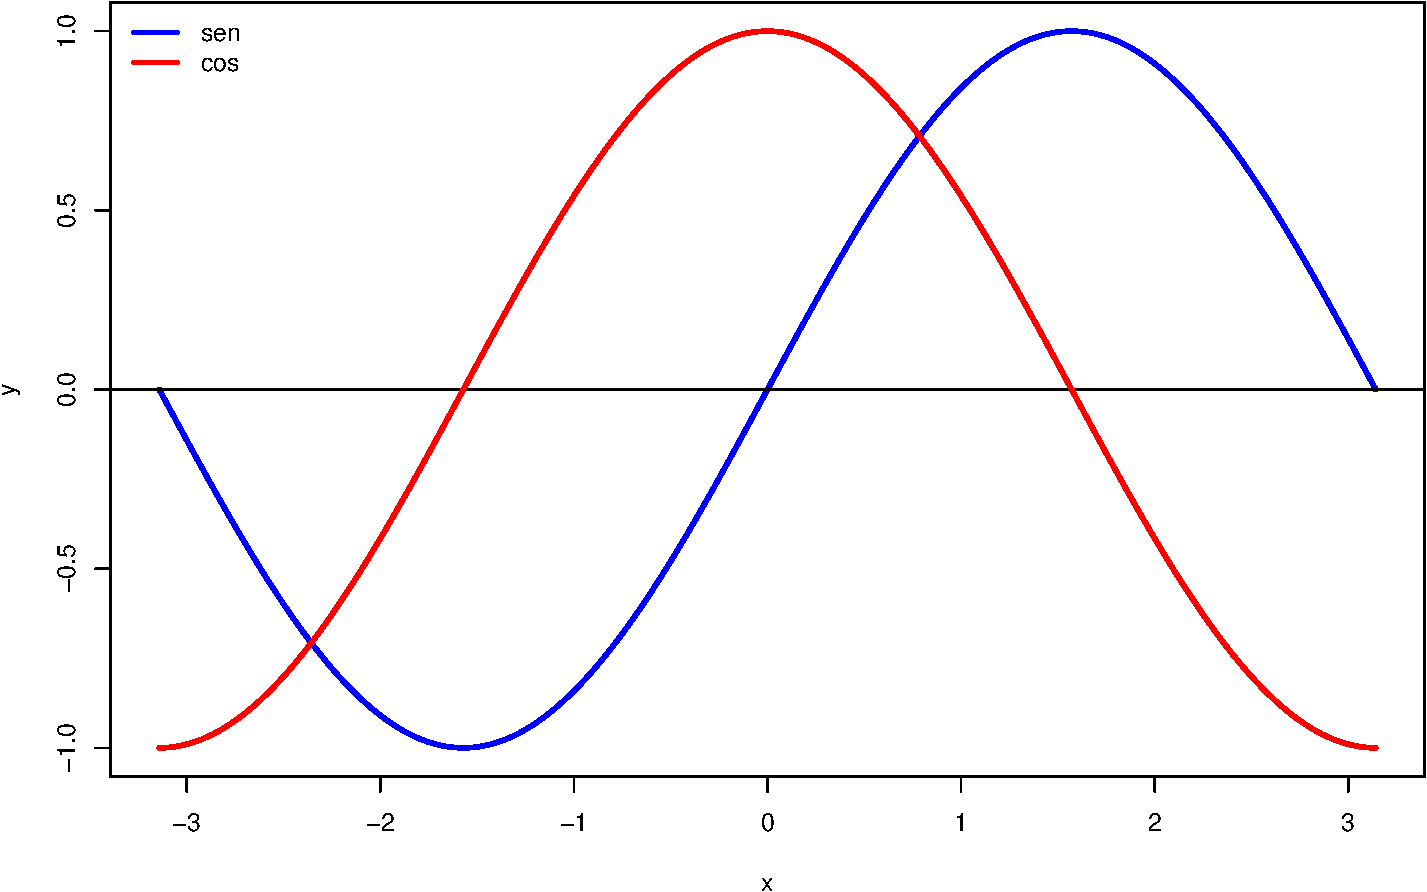
\includegraphics[keepaspectratio]{Clase1Calculdora_files/figure-beamer/unnamed-chunk-71-1.pdf}}
\end{frame}

\section{Mensajes de error}\label{mensajes-de-error}

\begin{frame}[fragile]{Mensajes de error}
\phantomsection\label{mensajes-de-error-1}
\begin{Shaded}
\begin{Highlighting}[]
\DocumentationTok{\#\#\# not run }
\FunctionTok{squareroot}\NormalTok{(}\DecValTok{4}\NormalTok{)  }\CommentTok{\# la función no existe }
\end{Highlighting}
\end{Shaded}

\begin{Shaded}
\begin{Highlighting}[]
\FunctionTok{lenght}\NormalTok{(}\FunctionTok{c}\NormalTok{(}\DecValTok{2}\NormalTok{,}\DecValTok{4}\NormalTok{,}\DecValTok{1}\NormalTok{)) }
\end{Highlighting}
\end{Shaded}

\begin{Shaded}
\begin{Highlighting}[]
\FunctionTok{length}\NormalTok{(}\DecValTok{2}\NormalTok{)}
\end{Highlighting}
\end{Shaded}

\begin{verbatim}
[1] 1
\end{verbatim}

\begin{Shaded}
\begin{Highlighting}[]
\FunctionTok{length}\NormalTok{(}\FunctionTok{c}\NormalTok{(}\DecValTok{1}\NormalTok{,}\DecValTok{5}\NormalTok{,}\DecValTok{6}\NormalTok{,}\DecValTok{9}\NormalTok{))}
\end{Highlighting}
\end{Shaded}

\begin{verbatim}
[1] 4
\end{verbatim}

\begin{Shaded}
\begin{Highlighting}[]
\FunctionTok{length}\NormalTok{(}\DecValTok{2}\NormalTok{)}
\end{Highlighting}
\end{Shaded}

\begin{verbatim}
[1] 1
\end{verbatim}

\begin{Shaded}
\begin{Highlighting}[]
\NormalTok{sqrt }\DecValTok{4}         \CommentTok{\# falta el parentesis }
\end{Highlighting}
\end{Shaded}

\begin{Shaded}
\begin{Highlighting}[]
\FunctionTok{sqrt}\NormalTok{(}\DecValTok{4} 
\end{Highlighting}
\end{Shaded}

\begin{Shaded}
\begin{Highlighting}[]
\NormalTok{y}\OtherTok{\textless{}{-}}\FunctionTok{sqrt}\NormalTok{(}\SpecialCharTok{{-}}\DecValTok{2}\NormalTok{) }
\NormalTok{x}\OtherTok{\textless{}{-}}\DecValTok{5}\SpecialCharTok{/}\DecValTok{0}
\end{Highlighting}
\end{Shaded}
\end{frame}

\begin{frame}[fragile]{Mensajes de error (II)}
\phantomsection\label{mensajes-de-error-ii}
\begin{Shaded}
\begin{Highlighting}[]
\NormalTok{x}
\end{Highlighting}
\end{Shaded}

\begin{verbatim}
[1] Inf
\end{verbatim}

\begin{Shaded}
\begin{Highlighting}[]
\NormalTok{y}
\end{Highlighting}
\end{Shaded}

\begin{verbatim}
[1] NaN
\end{verbatim}

\begin{Shaded}
\begin{Highlighting}[]
\FunctionTok{sqrt}\NormalTok{(}\SpecialCharTok{{-}}\DecValTok{2}\SpecialCharTok{+}\DecValTok{0}\NormalTok{i)}
\end{Highlighting}
\end{Shaded}

\begin{verbatim}
[1] 0+1.414214i
\end{verbatim}
\end{frame}

\section{Redondeo}\label{redondeo}

\begin{frame}[fragile]{Funciones para redondeo}
\phantomsection\label{funciones-para-redondeo}
\begin{Shaded}
\begin{Highlighting}[]
\CommentTok{\# al entero más cercano }
\FunctionTok{round}\NormalTok{(}\FloatTok{127.8976}\NormalTok{)}
\end{Highlighting}
\end{Shaded}

\begin{verbatim}
[1] 128
\end{verbatim}

\begin{Shaded}
\begin{Highlighting}[]
\FunctionTok{round}\NormalTok{(}\FloatTok{127.4999}\NormalTok{)}
\end{Highlighting}
\end{Shaded}

\begin{verbatim}
[1] 127
\end{verbatim}

\begin{Shaded}
\begin{Highlighting}[]
\CommentTok{\# redondeo a tres cifras significativas }
\FunctionTok{round}\NormalTok{(}\FloatTok{127.8976}\NormalTok{,}\DecValTok{3}\NormalTok{)}
\end{Highlighting}
\end{Shaded}

\begin{verbatim}
[1] 127.898
\end{verbatim}

\begin{Shaded}
\begin{Highlighting}[]
\DocumentationTok{\#\# piso }
\FunctionTok{floor}\NormalTok{(}\FloatTok{6.3}\NormalTok{) }\CommentTok{\# mayor entero que es menor que 6.3}
\end{Highlighting}
\end{Shaded}

\begin{verbatim}
[1] 6
\end{verbatim}

\begin{Shaded}
\begin{Highlighting}[]
\FunctionTok{floor}\NormalTok{(}\SpecialCharTok{{-}}\FloatTok{5.8}\NormalTok{)}
\end{Highlighting}
\end{Shaded}

\begin{verbatim}
[1] -6
\end{verbatim}
\end{frame}

\begin{frame}[fragile]{Funciones para redondeo (II)}
\phantomsection\label{funciones-para-redondeo-ii}
\begin{Shaded}
\begin{Highlighting}[]
\DocumentationTok{\#\# Techo  }
\FunctionTok{ceiling}\NormalTok{(}\FloatTok{6.3}\NormalTok{) }\CommentTok{\# menor entero que es mayor  que 6.3}
\end{Highlighting}
\end{Shaded}

\begin{verbatim}
[1] 7
\end{verbatim}

\begin{Shaded}
\begin{Highlighting}[]
\FunctionTok{ceiling}\NormalTok{(}\SpecialCharTok{{-}}\FloatTok{5.8}\NormalTok{)}
\end{Highlighting}
\end{Shaded}

\begin{verbatim}
[1] -5
\end{verbatim}
\end{frame}

\begin{frame}[fragile]{Vectores y asignaciones}
\phantomsection\label{vectores-y-asignaciones}
R opera sobre estructuras de datos con nombre. La estructura más simple
de este tipo es el vector, que es una entidad única que consta de una
colección ordenada datos. Los vectores son la estructura fundamental de
datos en R, un número es en realidad un vector de longitud 1. En cuanto
al contenido, hay tres tipos principales de vectores, a saber:

\begin{itemize}
\tightlist
\item
  Numéricos (numerical), los cuales pueden ser:

  \begin{itemize}
  \tightlist
  \item
    De reales (Double), la opción por defecto.
  \item
    De enteros (Integer) para compatibilidad con otros leguajes.
  \end{itemize}
\item
  De caracteres (Character)
\item
  Lógicos (Logical)
\end{itemize}

A continuación se crea el objeto (vector) \texttt{x} al cual se le
\texttt{asigna} el valor de 2,

\begin{Shaded}
\begin{Highlighting}[]
\NormalTok{x}\OtherTok{=}\DecValTok{2}
\FunctionTok{mode}\NormalTok{(x)}
\end{Highlighting}
\end{Shaded}

\begin{verbatim}
[1] "numeric"
\end{verbatim}

\begin{Shaded}
\begin{Highlighting}[]
\FunctionTok{class}\NormalTok{(x)}
\end{Highlighting}
\end{Shaded}

\begin{verbatim}
[1] "numeric"
\end{verbatim}

\begin{Shaded}
\begin{Highlighting}[]
\FunctionTok{typeof}\NormalTok{(x)}
\end{Highlighting}
\end{Shaded}

\begin{verbatim}
[1] "double"
\end{verbatim}

\begin{Shaded}
\begin{Highlighting}[]
\CommentTok{\# crea el objeto (vector) z  y se le asigna el valor de 5}
\NormalTok{z}\OtherTok{=}\DecValTok{5}
\end{Highlighting}
\end{Shaded}
\end{frame}

\begin{frame}[fragile]{Funcion \texttt{assign()}}
\phantomsection\label{funcion-assign}
Otra forma de asignar es con \texttt{assign()} de la siguiente manera.

\begin{Shaded}
\begin{Highlighting}[]
\FunctionTok{assign}\NormalTok{(}\StringTok{"y"}\NormalTok{, }\FunctionTok{c}\NormalTok{(}\DecValTok{4}\NormalTok{,}\FloatTok{1.2}\NormalTok{,}\DecValTok{3}\NormalTok{,}\FloatTok{2.5}\NormalTok{,}\DecValTok{6}\NormalTok{) )}
\DocumentationTok{\#\#\# equivalente a }
\NormalTok{y}\OtherTok{\textless{}{-}}\FunctionTok{c}\NormalTok{(}\DecValTok{4}\NormalTok{,}\FloatTok{1.2}\NormalTok{,}\DecValTok{3}\NormalTok{,}\FloatTok{2.5}\NormalTok{,}\DecValTok{6}\NormalTok{)}
\DocumentationTok{\#\#\# equivalente a }
\NormalTok{y}\OtherTok{=}\FunctionTok{c}\NormalTok{(}\DecValTok{4}\NormalTok{,}\FloatTok{1.2}\NormalTok{,}\DecValTok{3}\NormalTok{,}\FloatTok{2.5}\NormalTok{,}\DecValTok{6}\NormalTok{)}
\end{Highlighting}
\end{Shaded}
\end{frame}

\begin{frame}[fragile]{Aplicación}
\phantomsection\label{aplicaciuxf3n-1}
Graficar la función de densidad normal estándar

\begin{Shaded}
\begin{Highlighting}[]
\NormalTok{x}\OtherTok{\textless{}{-}}\FunctionTok{pretty}\NormalTok{(}\FunctionTok{c}\NormalTok{(}\SpecialCharTok{{-}}\DecValTok{3}\NormalTok{,}\DecValTok{3}\NormalTok{),}\DecValTok{100}\NormalTok{)}
\NormalTok{y}\OtherTok{\textless{}{-}}\FunctionTok{dnorm}\NormalTok{(x)}
\FunctionTok{plot}\NormalTok{(x,y,}\AttributeTok{type=}\StringTok{"l"}\NormalTok{)}
\end{Highlighting}
\end{Shaded}

\pandocbounded{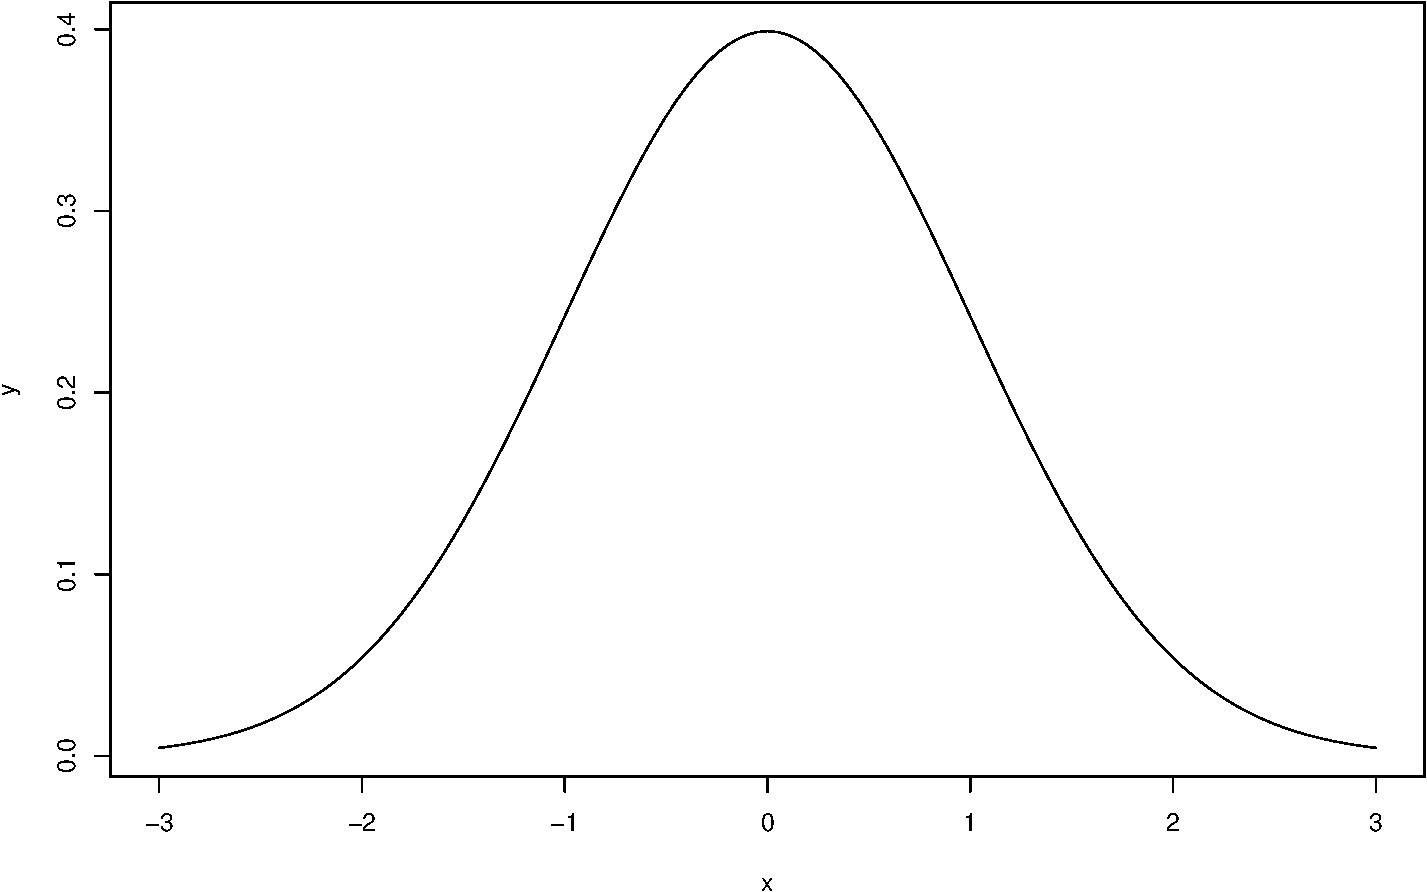
\includegraphics[keepaspectratio]{Clase1Calculdora_files/figure-beamer/unnamed-chunk-86-1.pdf}}
\end{frame}

\begin{frame}[fragile]{Aplicación}
\phantomsection\label{aplicaciuxf3n-2}
\begin{Shaded}
\begin{Highlighting}[]
\NormalTok{x}\OtherTok{\textless{}{-}}\FunctionTok{pretty}\NormalTok{(}\FunctionTok{c}\NormalTok{(}\SpecialCharTok{{-}}\DecValTok{3}\NormalTok{,}\DecValTok{3}\NormalTok{),}\DecValTok{100}\NormalTok{)}
\NormalTok{y}\OtherTok{\textless{}{-}}\FunctionTok{dnorm}\NormalTok{(x)}
\NormalTok{z}\OtherTok{\textless{}{-}}\FunctionTok{rnorm}\NormalTok{(}\DecValTok{100}\NormalTok{)}
\FunctionTok{hist}\NormalTok{(z,}\AttributeTok{freq=}\ConstantTok{FALSE}\NormalTok{,}\AttributeTok{ylim=}\FunctionTok{range}\NormalTok{(y))}
\FunctionTok{lines}\NormalTok{(x,y, }\AttributeTok{col=}\StringTok{"red"}\NormalTok{,}\AttributeTok{lwd=}\DecValTok{2}\NormalTok{)}
\end{Highlighting}
\end{Shaded}

\pandocbounded{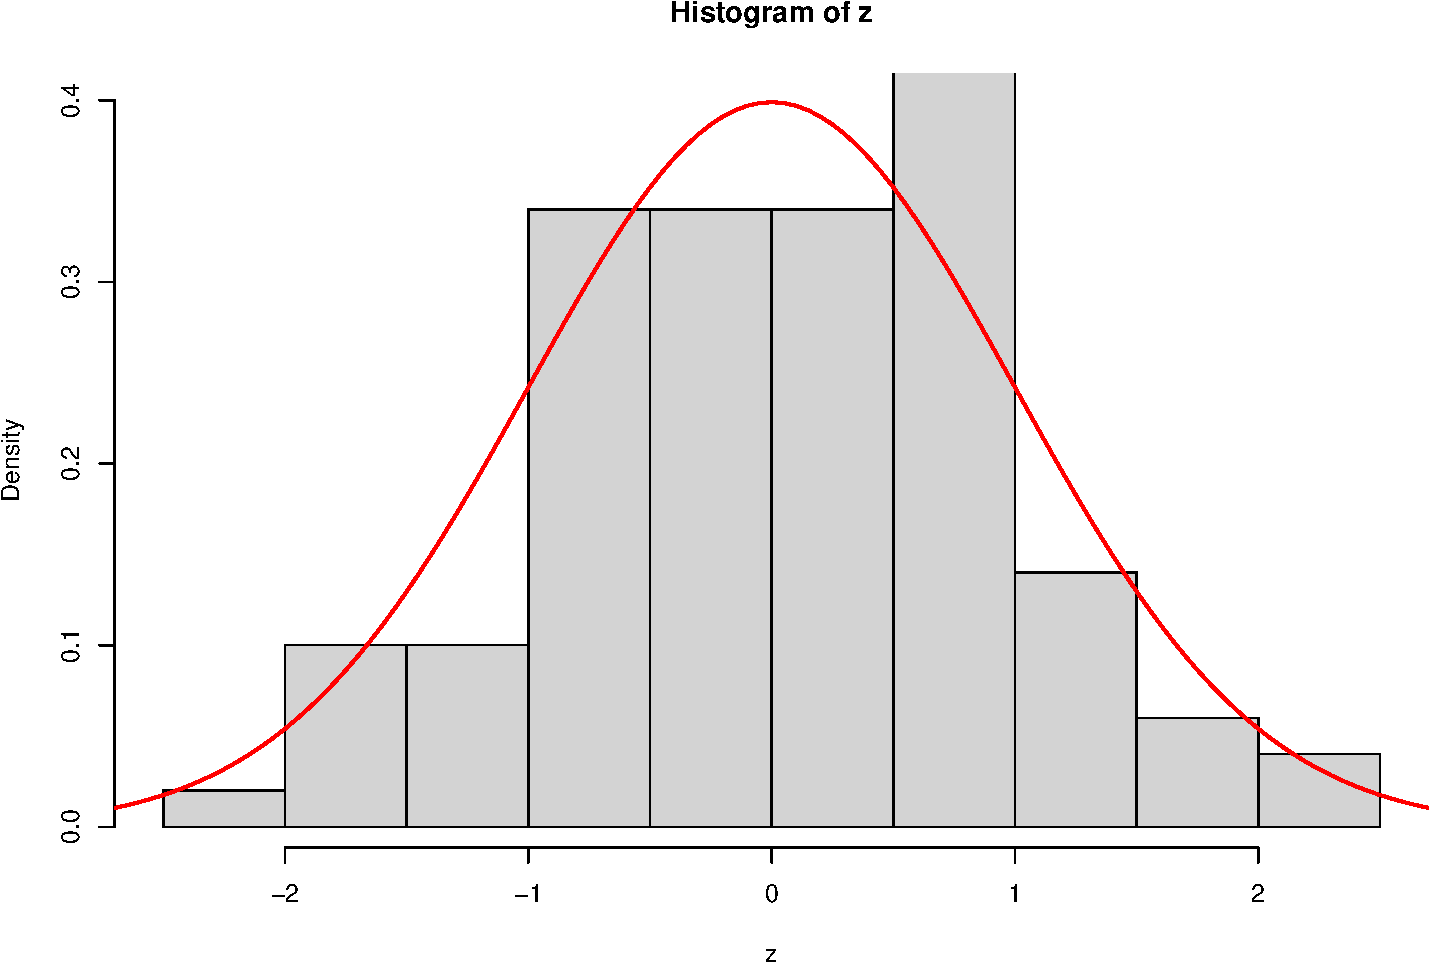
\includegraphics[keepaspectratio]{Clase1Calculdora_files/figure-beamer/unnamed-chunk-87-1.pdf}}
\end{frame}

\section{Caracteres}\label{caracteres-1}

\begin{frame}[fragile]{Vectores de caracteres}
\phantomsection\label{vectores-de-caracteres}
¿Qué objetos tengo en memoria?

\begin{Shaded}
\begin{Highlighting}[]
\NormalTok{ch}\OtherTok{\textless{}{-}}\FunctionTok{ls}\NormalTok{() }
\NormalTok{ch}
\end{Highlighting}
\end{Shaded}

\begin{verbatim}
[1] "x"  "y"  "y1" "z" 
\end{verbatim}

\begin{Shaded}
\begin{Highlighting}[]
\CommentTok{\#mode(ch)}
\CommentTok{\#typeof(ch)}
\FunctionTok{class}\NormalTok{(ch)}
\end{Highlighting}
\end{Shaded}

\begin{verbatim}
[1] "character"
\end{verbatim}

\begin{Shaded}
\begin{Highlighting}[]
\FunctionTok{is.character}\NormalTok{(ch)}
\end{Highlighting}
\end{Shaded}

\begin{verbatim}
[1] TRUE
\end{verbatim}

El objeto \texttt{ch} es un ejemplo de vector de caracteres.

Si el resultado de un calculo no se asigna, este se imprime y se pierde
(no se conserva en ningún objeto)
\end{frame}

\begin{frame}[fragile]{Vectores lógicos}
\phantomsection\label{vectores-luxf3gicos}
¿Las componentes del vector son iguales a 3?

\begin{Shaded}
\begin{Highlighting}[]
\FunctionTok{c}\NormalTok{(}\ConstantTok{TRUE}\NormalTok{,}\ConstantTok{FALSE}\NormalTok{,}\ConstantTok{TRUE}\NormalTok{)}
\end{Highlighting}
\end{Shaded}

\begin{verbatim}
[1]  TRUE FALSE  TRUE
\end{verbatim}

\begin{Shaded}
\begin{Highlighting}[]
\NormalTok{l}\OtherTok{=}\FunctionTok{c}\NormalTok{(}\DecValTok{3}\NormalTok{, }\DecValTok{4} \SpecialCharTok{{-}} \DecValTok{1}\NormalTok{, }\DecValTok{1} \SpecialCharTok{+} \DecValTok{1} \SpecialCharTok{+} \DecValTok{1}\NormalTok{,}\DecValTok{5}\SpecialCharTok{+}\DecValTok{2}\NormalTok{) }\SpecialCharTok{==} \DecValTok{3} 
\NormalTok{l}
\end{Highlighting}
\end{Shaded}

\begin{verbatim}
[1]  TRUE  TRUE  TRUE FALSE
\end{verbatim}

\begin{Shaded}
\begin{Highlighting}[]
\FunctionTok{mode}\NormalTok{(l)}
\end{Highlighting}
\end{Shaded}

\begin{verbatim}
[1] "logical"
\end{verbatim}

\begin{Shaded}
\begin{Highlighting}[]
\FunctionTok{typeof}\NormalTok{(l)}
\end{Highlighting}
\end{Shaded}

\begin{verbatim}
[1] "logical"
\end{verbatim}

\begin{Shaded}
\begin{Highlighting}[]
\FunctionTok{class}\NormalTok{(l)}
\end{Highlighting}
\end{Shaded}

\begin{verbatim}
[1] "logical"
\end{verbatim}

El anterior es un ejemplo de un vector lógico
\end{frame}




\end{document}
